% **** Szablon pracy magisterskiej, licencjackiej lub inżynierskiej ****

\documentclass[polish,12pt,twoside,a4paper]{report}

% *************** Definicje stylu dokumentu ***************

% *********************************************************************************
% W pliku tym zdefiniowany jest wygl¹d dokumentu.
% Zmiany tutaj nie s¹ konieczne o ile nie zamierzasz zmieniaæ wygl¹du dokumentu.
% *********************************************************************************

% *************** Za³adowanie pakietów ***************
\usepackage[a4paper,twoside,left=2.0cm,right=1.5cm,top=1.5cm,bottom=1.5cm]{geometry}
\usepackage[T1]{fontenc}
%\usepackage[cp1250]{inputenc}
\usepackage[utf8]{inputenc}
\usepackage[polish]{babel}
\usepackage{amsmath}
\usepackage{amsfonts}
\usepackage{graphicx}
\usepackage{graphics}
\usepackage{times}
\usepackage{indentfirst}%wciecia a nowych akapitach

\selectlanguage{polish}

%szerokoœœ wciêæ
\setlength{\parindent}{1.25cm}

%numeracja stron
\usepackage{fancyhdr}
\pagestyle{fancy}
\fancyhf{} % usun biezace ustawienia pagin
\fancyhead[LE,RO]{ }
\fancyhead[LO]{ }
\fancyhead[RE]{ }
\fancyfoot[LE,RO]{\small\thepage}
\fancyfoot[LO]{ }
\fancyfoot[RE]{ }
\renewcommand{\headrulewidth}{0.0pt}
\renewcommand{\footrulewidth}{0.0pt}
\addtolength{\headheight}{0.0pt} % pionowy odstep na kreske
\fancypagestyle{plain}{%
\fancyhead{} % usun p. górne na stronach pozbawionych
% numeracji (plain)
\renewcommand{\headrulewidth}{0.0pt} % pozioma kreska
}

% *************** Definicje niektórych kolorów ***************
\usepackage{color}

\definecolor{greenyellow}   {cmyk}{0.15, 0   , 0.69, 0   }
\definecolor{yellow}        {cmyk}{0   , 0   , 1   , 0   }
\definecolor{goldenrod}     {cmyk}{0   , 0.10, 0.84, 0   }
\definecolor{dandelion}     {cmyk}{0   , 0.29, 0.84, 0   }
\definecolor{apricot}       {cmyk}{0   , 0.32, 0.52, 0   }
\definecolor{peach}         {cmyk}{0   , 0.50, 0.70, 0   }
\definecolor{melon}         {cmyk}{0   , 0.46, 0.50, 0   }
\definecolor{yelloworange}  {cmyk}{0   , 0.42, 1   , 0   }
\definecolor{orange}        {cmyk}{0   , 0.61, 0.87, 0   }
\definecolor{burntorange}   {cmyk}{0   , 0.51, 1   , 0   }
\definecolor{bittersweet}   {cmyk}{0   , 0.75, 1   , 0.24}
\definecolor{redorange}     {cmyk}{0   , 0.77, 0.87, 0   }
\definecolor{mahogany}      {cmyk}{0   , 0.85, 0.87, 0.35}
\definecolor{maroon}        {cmyk}{0   , 0.87, 0.68, 0.32}
\definecolor{brickred}      {cmyk}{0   , 0.89, 0.94, 0.28}
\definecolor{red}           {cmyk}{0   , 1   , 1   , 0   }
\definecolor{orangered}     {cmyk}{0   , 1   , 0.50, 0   }
\definecolor{rubinered}     {cmyk}{0   , 1   , 0.13, 0   }
\definecolor{wildstrawberry}{cmyk}{0   , 0.96, 0.39, 0   }
\definecolor{salmon}        {cmyk}{0   , 0.53, 0.38, 0   }
\definecolor{carnationpink} {cmyk}{0   , 0.63, 0   , 0   }
\definecolor{magenta}       {cmyk}{0   , 1   , 0   , 0   }
\definecolor{violetred}     {cmyk}{0   , 0.81, 0   , 0   }
\definecolor{rhodamine}     {cmyk}{0   , 0.82, 0   , 0   }
\definecolor{mulberry}      {cmyk}{0.34, 0.90, 0   , 0.02}
\definecolor{redviolet}     {cmyk}{0.07, 0.90, 0   , 0.34}
\definecolor{fuchsia}       {cmyk}{0.47, 0.91, 0   , 0.08}
\definecolor{lavender}      {cmyk}{0   , 0.48, 0   , 0   }
\definecolor{thistle}       {cmyk}{0.12, 0.59, 0   , 0   }
\definecolor{orchid}        {cmyk}{0.32, 0.64, 0   , 0   }
\definecolor{darkorchid}    {cmyk}{0.40, 0.80, 0.20, 0   }
\definecolor{purple}        {cmyk}{0.45, 0.86, 0   , 0   }
\definecolor{plum}          {cmyk}{0.50, 1   , 0   , 0   }
\definecolor{violet}        {cmyk}{0.79, 0.88, 0   , 0   }
\definecolor{royalpurple}   {cmyk}{0.75, 0.90, 0   , 0   }
\definecolor{blueviolet}    {cmyk}{0.86, 0.91, 0   , 0.04}
\definecolor{periwinkle}    {cmyk}{0.57, 0.55, 0   , 0   }
\definecolor{cadetblue}     {cmyk}{0.62, 0.57, 0.23, 0   }
\definecolor{cornflowerblue}{cmyk}{0.65, 0.13, 0   , 0   }
\definecolor{midnightblue}  {cmyk}{0.98, 0.13, 0   , 0.43}
\definecolor{navyblue}      {cmyk}{0.94, 0.54, 0   , 0   }
\definecolor{royalblue}     {cmyk}{1   , 0.50, 0   , 0   }
\definecolor{blue}          {cmyk}{1   , 1   , 0   , 0   }
\definecolor{cerulean}      {cmyk}{0.94, 0.11, 0   , 0   }
\definecolor{cyan}          {cmyk}{1   , 0   , 0   , 0   }
\definecolor{processblue}   {cmyk}{0.96, 0   , 0   , 0   }
\definecolor{skyblue}       {cmyk}{0.62, 0   , 0.12, 0   }
\definecolor{turquoise}     {cmyk}{0.85, 0   , 0.20, 0   }
\definecolor{tealblue}      {cmyk}{0.86, 0   , 0.34, 0.02}
\definecolor{aquamarine}    {cmyk}{0.82, 0   , 0.30, 0   }
\definecolor{bluegreen}     {cmyk}{0.85, 0   , 0.33, 0   }
\definecolor{emerald}       {cmyk}{1   , 0   , 0.50, 0   }
\definecolor{junglegreen}   {cmyk}{0.99, 0   , 0.52, 0   }
\definecolor{seagreen}      {cmyk}{0.69, 0   , 0.50, 0   }
\definecolor{green}         {cmyk}{1   , 0   , 1   , 0   }
\definecolor{forestgreen}   {cmyk}{0.91, 0   , 0.88, 0.12}
\definecolor{pinegreen}     {cmyk}{0.92, 0   , 0.59, 0.25}
\definecolor{limegreen}     {cmyk}{0.50, 0   , 1   , 0   }
\definecolor{yellowgreen}   {cmyk}{0.44, 0   , 0.74, 0   }
\definecolor{springgreen}   {cmyk}{0.26, 0   , 0.76, 0   }
\definecolor{olivegreen}    {cmyk}{0.64, 0   , 0.95, 0.40}
\definecolor{rawsienna}     {cmyk}{0   , 0.72, 1   , 0.45}
\definecolor{sepia}         {cmyk}{0   , 0.83, 1   , 0.70}
\definecolor{brown}         {cmyk}{0   , 0.81, 1   , 0.60}
\definecolor{tan}           {cmyk}{0.14, 0.42, 0.56, 0   }
\definecolor{gray}          {cmyk}{0   , 0   , 0   , 0.50}
\definecolor{black}         {cmyk}{0   , 0   , 0   , 1   }
\definecolor{white}         {cmyk}{0   , 0   , 0   , 0   } 

% *************** Koniec definicji stylu dokumentu ***************


%definicja przydatnych poleceń
\newcommand{\wydzial}{KOLEGIUM INFORMATYKI STOSOWANEJ}
\newcommand{\kierunek}{Kierunek: INFORMATYKA}
\newcommand{\specjalnosc}{Specjalność: Technologie internetowe i mobilne}
\newcommand{\autor}{Rafał Wąż}
\newcommand{\album}{Nr albumu studenta w67207}
\newcommand{\temat}{System Zarządzania Symulacją Samochodu}
\newcommand{\promotor}{mgr inż. Ewa Żesławska}
\newcommand{\typpracy}{Praca projektowa programowanie obiektowe C\#}
\newcommand{\miasto}{Rzeszów}
\newcommand{\rok}{2024}

\begin{document}

% *************** Włączenie definicji pierwszych stron ***************
% *************** Strony tytułowe ***************

% ************************************************************
% W tym miejscu znajduje sie definicja wyglądu pierwszych stron:
% strony tytułowej, strony z oświadczeniem o treści pracy
% i strony ze spisem treści
% ************************************************************
% *************** Strona tytułowa ***************
%umieszczenie logo i nazwy uczelni
\noindent
\parbox{65mm}{
\includegraphics[width=13.0cm, height=3.0cm]{logoWSIiZ}}

\vspace{10mm}
\begin{center}
{\Large{}\textbf{\wydzial}}
\end{center}
\vspace{10mm}
\noindent
\hspace{30mm}{\Large{}\textbf{\kierunek}}\\

\noindent
\hspace{30mm}{\Large{}\textbf{\specjalnosc}}
\vspace{30mm}
\begin{center}
	{\large{}\autor}\\
	{\large{}\album}\\
	\vspace{15pt}
	{\huge{}\textbf{\textit{\temat}}}\\
	\vspace{20pt}
	{\normalsize{}Promotor: \promotor}\\
	\vspace{100pt}
	{\LARGE{}\textbf{\typpracy}}\\
	\vspace{190pt}
	{\large{}\textbf{\miasto {} \rok}}
\end{center}

% pusta zawartość stopki - brak numeru strony
\thispagestyle{empty}

% *************** Strona z oświadczeniem o treści pracy ***************



% *************** Spis treści ***************
\tableofcontents
% pusta zawartość stopki - brak numeru strony
\thispagestyle{empty}
\newpage

% *************** Koniec pliku front.tex ***************


% *************** Część główna pracy ***************
\chapter*{Wstęp}

W dzisiejszych czasach, rozwój technologii motoryzacyjnych przynosi za sobą  nowe możliwości, jak i wyzwania związane z bezpieczeństwem na drogach. Testowanie zachowań samochodu w różnych warunkach drogowych staje się coraz bardziej istotne, zwłaszcza w kontekście wprowadzania zaawansowanych systemów wspomagających kierowcę. Projekt "System Zarządzania Symulacją Samochodu" powstał z myślą o stworzeniu kompleksowego narzędzia do symulowania oraz analizowania zachowania pojazdu.




\addcontentsline{toc}{chapter}{Wstęp}
\newpage
% ********** Rozdział 1 **********
\chapter{Opis założeń projektu}
\section{Założenia projektu}
\begin{itemize}
\item 
Projekt zakłada stworzenie realistycznego doświadczenia jazdy samochodem, umożliwiając jednocześnie symulację podstawowych funkcji pojazdu oraz monitorowanie kluczowych parametrów. Użytkownik będzie mógł interaktywnie kontrolować samochód, włączając i wyłączając silnik, zmieniając biegi, przyspieszając i hamując. Podczas symulacji będzie mógł również obserwować różne parametry pojazdu, takie jak aktualna prędkość, aktualny bieg i obroty silnika. Ponadto, program będzie obsługiwał sytuacje, w których jazda nie będzie możliwa ze względu na brak paliwa lub zatarty silnik. 
\end{itemize}

\section{Wymagania funkcjonalne i niefunkcjonalne}
\noindent{Wymagania funkcjonalne:}
\begin{itemize}
\item Symulacja działania samochodu: System będzie umożliwiał symulację różnych aspektów działania samochodu.
\item Monitorowanie zużycia paliwa: System umożliwia monitorowanie ilości zużytego paliwa w czasie rzeczywistym podczas symulacji.
\item Analiza efektywności spalania: System dostarcza analize efektywności spalania w różnych warunkach jazdy na podstawie zebranych danych.
\item Analiza kosztów: System przeprowadza analizę kosztów paliwa na podstawie zebranych danych symulacyjnych.
\item Obserwacja średniej prędkości podróży: System umożliwia obserwację średniej prędkości podróży i dostarczanie statystyk na temat czasu przebytej trasy.
\end{itemize}
\noindent{Wymagania niefunkcjonalne:}
\begin{itemize}
\item Wydajność: Aplikacja działa płynnie i dostarcza informacje w czasie rzeczywistym, zapewniając szybkie i efektywne działanie symulacji samochodu.
\item Intuicyjny interfejs: Interfejs aplikacji jest intuicyjny i łatwy w obsłudze, umożliwiając użytkownikowi wygodne korzystanie z funkcji symulacji samochodu.
\item Dostępność systemu: System zapewnia wysoką dostępność, umożliwiając korzystanie z funkcji symulacji samochodu przez większość czasu. 
\end{itemize}


% ********** Koniec rozdziału **********

\newpage
% ********** Rozdział 2 **********
\chapter{Realizacja projektu}


\section{Opis struktury projektu}

Projekt "System Zarządzania Symulacją Samochodu" zakłada stworzenie systemu, który będzie symulować działanie samochodu w różnych warunkach drogowych, umożliwiając testowanie i analizę jego zachowania w kontrolowanych warunkach.
\begin{itemize}
    \item Klasa Samochód: Odpowiada za symulację działania samochodu, w tym kontrolę prędkości, hamowania, uwzględniając parametry techniczne i zmiany prędkości obrotowej.
    \item Klasa Silnik: Symuluje zachowanie włączenie lub wyłączenie silnika samochodu, określenie poziomu paliwa stanu oleju.
    \item Klasa Skrzynia biegów: Zarządza zmianą biegów w samochodzie i dostosowuje prędkość obrotową silnika do aktualnych warunków jazdy.
    \item Klasa Parametry: Przechowuje parametry samochodu, takie jak maksymalna prędkość, pojemność baku paliwa, średnie spalanie.
    \item Klasa Zużycie paliwa: Odpowiada za monitorowanie zużycia paliwa przez samochód w trakcie symulacji.
    \item Klasa Trasa: Symuluje trasę, po której porusza się samochód, uwzględniając różne warunki takiej jak odległość, czas podróży, średnia prędkość oraz punkt docelowy.
    \item Klasa Koszty: Zarządza obliczaniem kosztów podróży na podstawie zużycia paliwa i innych czynników.
    \item Klasa Program: Punkt wejścia do aplikacji, odpowiedzialny za uruchomienie symulacji oraz inicjalizację pozostałych komponentów.
\end{itemize}

W następnej części projektu został opracowany diagram klas, który przedstawia strukturę klas i ich relacje w ramach systemu. Diagram klas pozwala zobaczyć, jak poszczególne klasy są ze sobą powiązane, jakie są ich właściwości i metody oraz w jaki sposób komunikują się między sobą.

\begin{figure}[!ht]
	\centering
		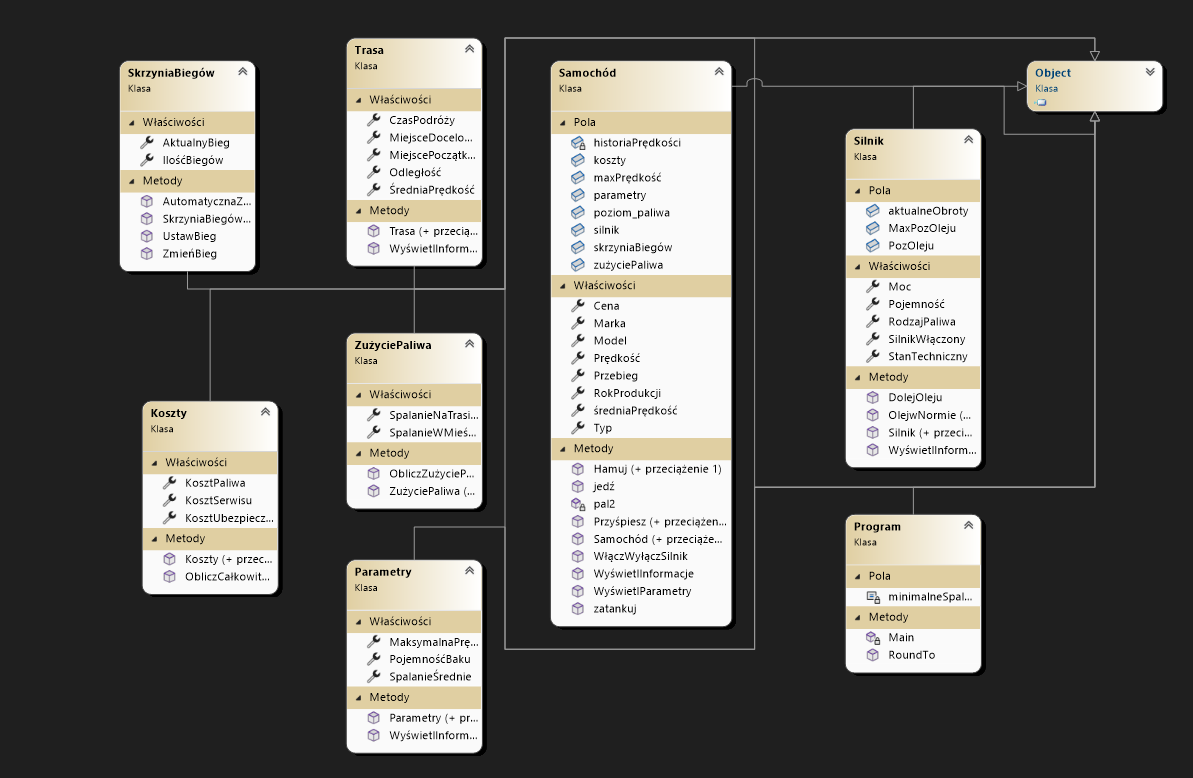
\includegraphics[width=16cm]{Diagram klas.png}
	\caption{\footnotesize Diagram klas}
	\label{fig:plotend}
\end{figure}
\newpage
\section{Opis techniczny projektu}

Projekt "System Zarządzania Symulacją Samochodu" ma na celu stworzenie kompleksowego systemu do symulacji oraz analizy zachowania pojazdu. System ten umożliwi użytkownikom interaktywne sterowanie symulowanym samochodem, monitorowanie kluczowych parametrów oraz przeprowadzanie analiz efektywności spalania, kosztów eksploatacji i innych istotnych wskaźników.
\begin{itemize}
\item .NET Framework: .NET Framework to fundamentalna platforma programistyczna, umożliwiająca rozwój różnorodnych aplikacji w języku C\# oraz innych obsługiwanych językach. Zapewnia szeroki zakres bibliotek i narzędzi, które ułatwiają tworzenie aplikacji desktopowych, webowych, serwerowych i innych. Dzięki swojej wszechstronności, .NET Framework umożliwia szybkie i efektywne rozwijanie oprogramowania.
\item Visual Studio: Visual Studio to kompleksowe środowisko programistyczne firmy Microsoft, które oferuje narzędzia do tworzenia, testowania, debugowania i zarządzania projektami. Dzięki zaawansowanym funkcjom, Visual Studio znacząco zwiększa produktywność i ułatwia rozwój aplikacji.
\item GitHub: GitHub to platforma hostingowa oparta na systemie kontroli wersji Git, która umożliwia przechowywanie kodu źródłowego, śledzenie zmian oraz współpracę zespołową nad projektem. 

Minimalne wymagania systemowe:
\begin{itemize}
    \item \textbf{System operacyjny:} Windows 10, macOS, Linux 
    \item \textbf{Procesor:} ARM64 lub x64; Zalecany czterordzeniowy lub lepszy.
    \item \textbf{Pamięć RAM:} Zalecane 4 procesory wirtualne i 16 GB pamięci RAM
    \item \textbf{Miejsce na dysku twardym:} minimalnie 850 MB
    \item \textbf{.NET:} .NET Framework lub .NET Core
\end{itemize}
\end{itemize}
\section{Zarządzanie danymi }
\begin{figure}[!ht]
	\centering
		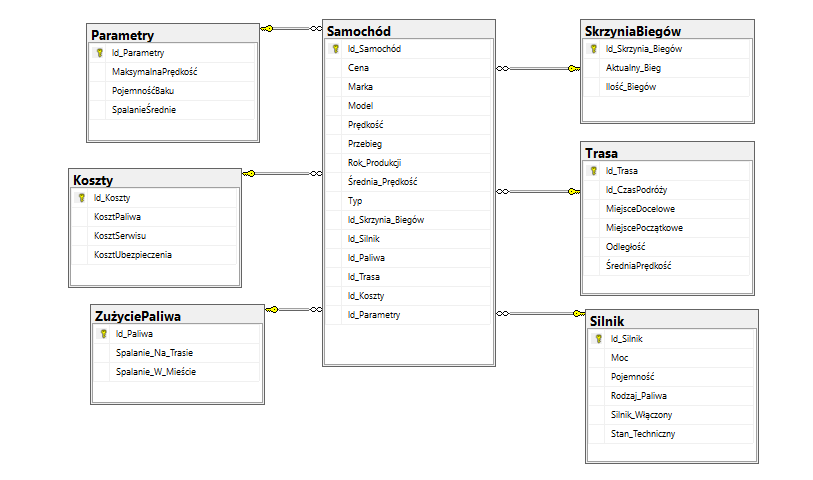
\includegraphics[width=14cm]{bazy danych.png}
	\caption{\footnotesize Schemat bazy danych}
	\label{fig:plotend}
\end{figure}
\begin{itemize}
    \item Samochód: Tabela Samochód pełni kluczową rolę jako główna tabela, łącząc relacje z innymi tabelami w systemie. Służy do przechowywania danych o samochodzie oraz zawiera klucze obce, które odnoszą się do innych istotnych aspektów pojazdu. Klucze obce umożliwiają powiązanie informacji o samochodzie z różnymi aspektami, takimi jak informacje o silniku, zużyciu paliwa, skrzyni biegów, trasy podróży, koszty eksploatacji oraz parametry techniczne. 
    \item Silnik: Tabela Silnik jest istotna dla systemu zarządzania pojazdu, ponieważ przechowuje kluczowe informacje o silniku samochodowym, co umożliwia monitorowanie ich parametrów technicznych oraz planowanie konserwacji i napraw.
    \item SkrzyniaBiegów: Tabela SkrzyniaBiegów przechowuje kluczowe informacje o skrzyni biegów w samochodzie. Te dane mogą być używane do monitorowania aktualnego biegu oraz analizy charakterystyki jazdy pojazdu.
    \item ZużyciePaliwa: Tabela ZużyciePaliwa umożliwia śledzenie zużycia paliwa przez samochód w różnych warunkach, takich jak jazda w terenie miejskim i na trasie. Informacje są istotne dla monitorowania wydajności samochodu pod względem zużycia paliwa.
    \item Trasa: Tabela Trasa umożliwia śledzenie informacji o poszczególnych trasach podróży samochodowych, dane dotyczące miejsc początkowych i docelowych, odległości pokonanej trasy oraz średniej prędkości podróżowania.
    \item Parametry: Tabela Parametry zawiera istotne informacje dotyczące parametrów technicznych samochodów, takich jak maksymalna prędkość, pojemność baku oraz średnie spalanie paliwa. 
    \item Koszty: Tabela Koszty umożliwia śledzenie kosztów związanych z eksploatacją samochodu.
\end{itemize}
% ********** Koniec rozdziału **********

\newpage
% ********** Rozdział 3 **********
\chapter{Przedstawienie realizacji projektu}
\section{Realizacja projektu}
Przedstawienie realizacji projektu "System Zarządzania Symulacją Samochodu" jest stworzony w programie Visual Studio 2022 w języku C\#. W tej części przedstawiam diagram Gantta.
\begin{figure}[!ht]
	\centering
		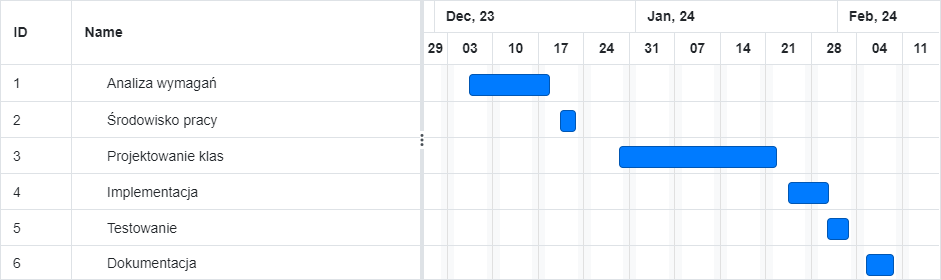
\includegraphics[width=17cm]{Diagram Gantta.png}
	\caption{\footnotesize Diagram Gantta}
	\label{fig:plotend}
\end{figure}

\begin{itemize}
\item Analiza wymagań: Proces polegający na ustaleniu konkretnych wymagań dla systemu zarządzania symulacją samochodu. Wymaga to dokładne zrozumienie i zebranie informacji potrzebnych do działania aplikacji.
\item Środowisko pracy: To miejsce, w którym przygotowuje się stanowisko programistyczne poprzez zainstalowanie odpowiednich pakietów środowiska i narzędzi na komputerze. Po przygotowaniu można przystąpić do tworzenia projektu.
\item Projektowanie klas: Etap projektowania obiektowego, podczas którego definiuje się klasy, ich właściwości i metody, aby zorganizować i strukturyzować kod źródłowy. W przypadku symulacji zachowania samochodu może to obejmować klasy reprezentujące różne aspekty samochodu.
\item Implenetacja: Proces przekształcania projektu i koncepcji klas w działający kod źródłowy, który realizuje określone funkcjonalności i spełnia wymagania użytkowników. W symulacji zachowania samochodu może to oznaczać implementację logiki sterującej zachowaniem samochodu.
\item Testowanie: Proces sprawdzania poprawności i skuteczności aplikacji poprzez wykonywanie testów na różnych etapach tworzenia. Testowanie symulacji zachowania samochodu może obejmować symulację różnych scenariuszy drogowych i sprawdzenie, czy samochód zachowuje się zgodnie z oczekiwaniami.
\item Dokumentacja: Tworzenie dokumentacji, która opisuje projekt, jego funkcjonalności, strukturę kodu źródłowego, sposób korzystania z aplikacji 
\end{itemize}

\section{Repozytorium i system kontroli wersji}
Projekt znajdujący się na stronie GitHub posiada wiele możliwości, które mogą być wykorzystane w celu monitorowania kodu.
Repozytorium znajduje się pod adresem:

\textbf {https://github.com/rafalwaz/System-zarzadzania-symulacja-samochodu}

\section{Prezentacja warstwy użytkowej projektu}
Zaprojektowanie warstwy użytkowej projektu "System Zarządzania Symulacją Samochodu" w sposób prosty, czytelny i łatwy dla użytkownika oraz wyeksponowanie funkcji działania rzeczywistej symulacji w interfejsie są kluczowe dla zapewnienia płynnej interakcji oraz maksymalnego zrozumienia procesu symulacji przez użytkowników. Ten podejście pozwoli użytkownikom szybko i efektywnie korzystać z systemu, co z kolei zwiększy ich satysfakcję i zaufanie do jego możliwości.

\begin{figure}[!ht]
	\centering
		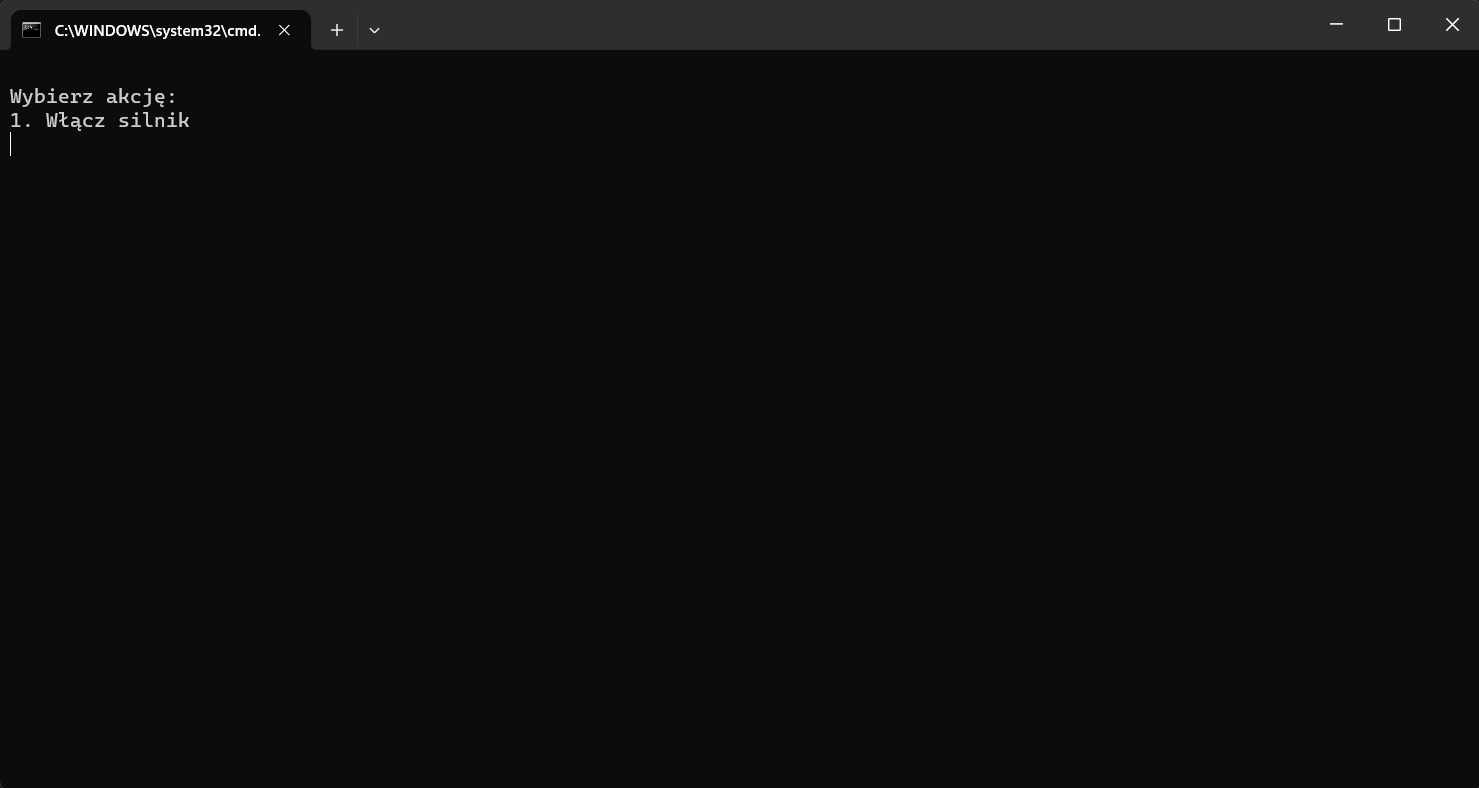
\includegraphics[width=17cm]{Włącz silnik.png}
	\caption{\footnotesize Włącz silnik}
	\label{fig:plotend}
\end{figure}

Uruchamiając program w konsoli wyświetla się informacja, która za pomocą przycisku numer 1 na klawiaturze wybierze akcje włącz silnik.
\newpage
Po wybraniu opcji na klawiaturze, użytkownik widzi w aplikacji włączony silnik, stan oleju, stan paliwa, pojemność w baku, aktulany stan silnika, aktualny bieg, prędkość, obroty silnika, ilość paliwa. 

\begin{figure}[!ht]
	\centering
		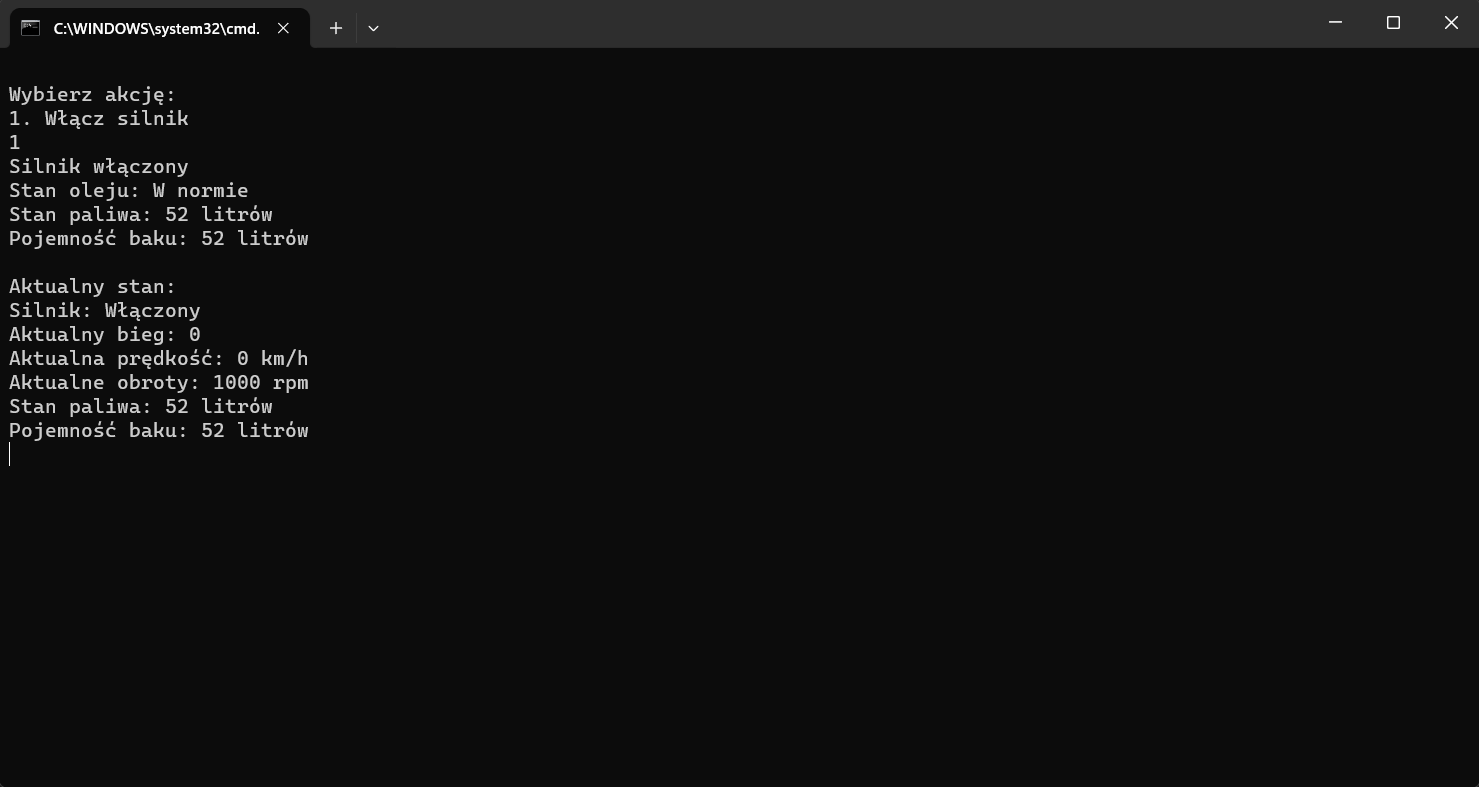
\includegraphics[width=17cm]{Włączony silnik.png}
	\caption{\footnotesize Włączony silnik}
	\label{fig:plotend}
\end{figure}
 
W sytuacji kiedy chcemy rozpocząć jazde na konsoli jest do wyboru opcja numer 2 która wskazuje przyśpieszenie samochodu 

\begin{figure}[!ht]
	\centering
		\includegraphics[width=17cm]{Wybór akcji.png}
	\caption{\footnotesize Wybór akcji}
	\label{fig:plotend}
\end{figure}

\newpage
Następnie w konsoli wystąpiła zmiana, kiedy przyśpieszono aktualna prędkość osiągneła 10km/h.  

\begin{figure}[!ht]
	\centering
		\includegraphics[width=17cm]{Przyśpieszenie.png}
	\caption{\footnotesize Przyśpieszenie}
	\label{fig:plotend}
\end{figure}
W konsoli wystąpiła zmiana aktualnie samochód porusza się na trzecim biegu. 
\begin{figure}[!ht]
	\centering
		\includegraphics[width=17cm]{Zmiana biegów.png}
	\caption{\footnotesize Zmiana biegów}
	\label{fig:plotend}
\end{figure}
\newpage
Aktualna prędkość 100km/h, zużycie paliwa 0,1 litrów. Na piątym biegu obroty silnika w tym momencie mają 3100 rpm. Stan paliwa na ten moment wynosi 41,9 litrów. Zużycie paliwa przy tej prędkości pokazuje 0,1 litrów, na takiej jeździe przewidywana ilość kilometrów na aktualnym stanie paliwa przewiduje 471km.
W przypadku kiedy trasa od Rzeszowa do Kielnarowej wynosi 17km przy prędkości 100km/h, średnia prędkość w przybliżeniu jest 86,84 km/h natomiast czas podróży będzie wynosił 11 minut 44 sekundy.

\begin{figure}[!ht]
	\centering
		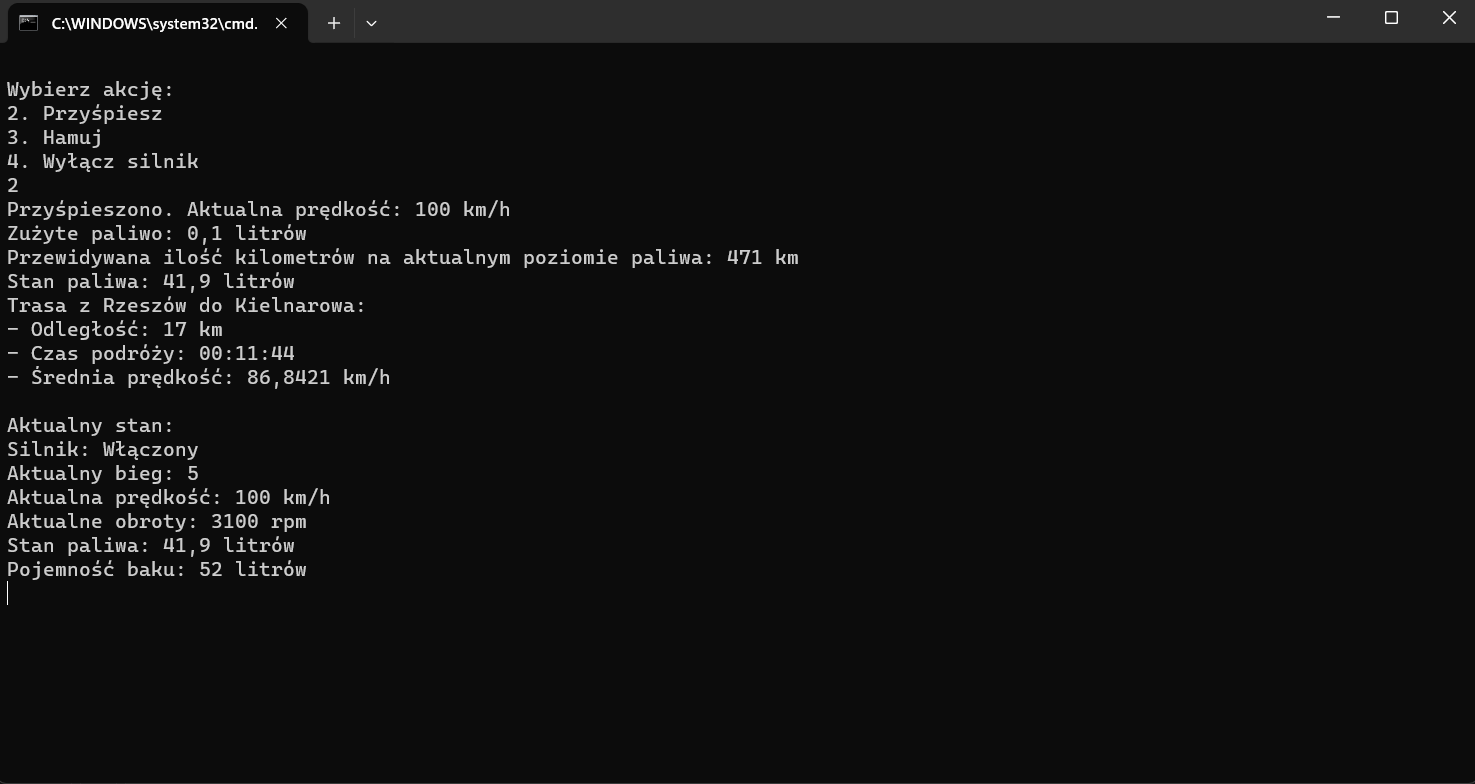
\includegraphics[width=17cm]{Parametry.png}
	\caption{\footnotesize Wyświetlenie parametrów}
	\label{fig:plotend}
\end{figure}

Jeżeli na konsoli użytkownik wybierze akcję numer 3, spowoduje hamowanie samochodu i automatycznie spadną obroty silnika i prędkość oraz bieg w tym przypadku zostanie zmieniony o jeden mniejszy. 

\begin{figure}[!ht]
	\centering
		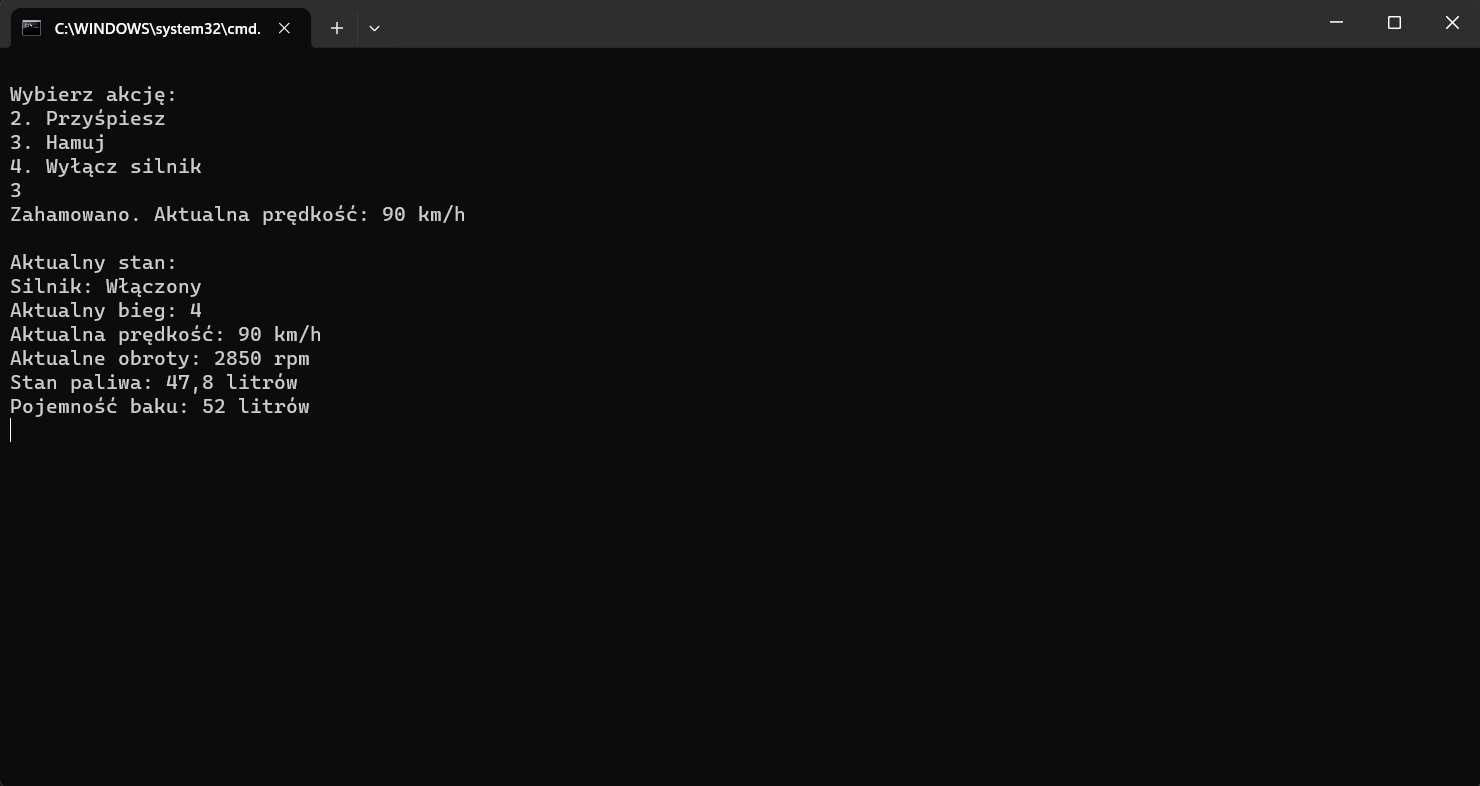
\includegraphics[width=17cm]{Hamowanie.png}
	\caption{\footnotesize Hamowanie}
	\label{fig:plotend}
\end{figure}
\newpage
W przypadku kiedy użytkownik zużyje paliwo a stan paliwa będzie wynosił 0 litrów. Wyświetli się informacja o braku paliwa i tym samym dalsza jazda nie będzie możliwa.

\begin{figure}[!ht]
	\centering
		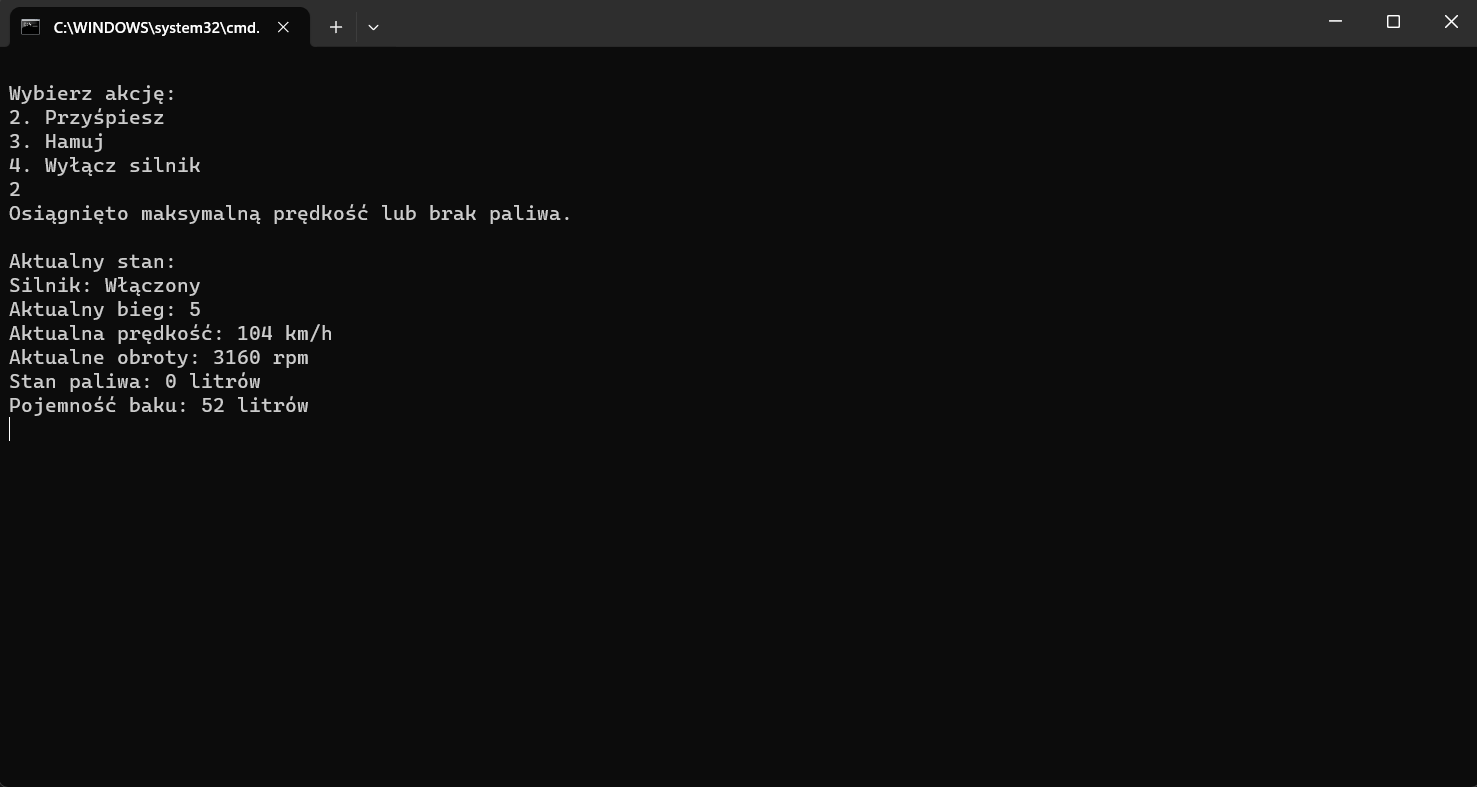
\includegraphics[width=17cm]{Brak paliwa.png}
	\caption{\footnotesize Brak paliwa}
	\label{fig:plotend}
\end{figure}

Kiedy użytkownik chce zakończyć jazde na consoli wybierze akcję numer 4 wyłącz silnik.

\begin{figure}[!ht]
	\centering
		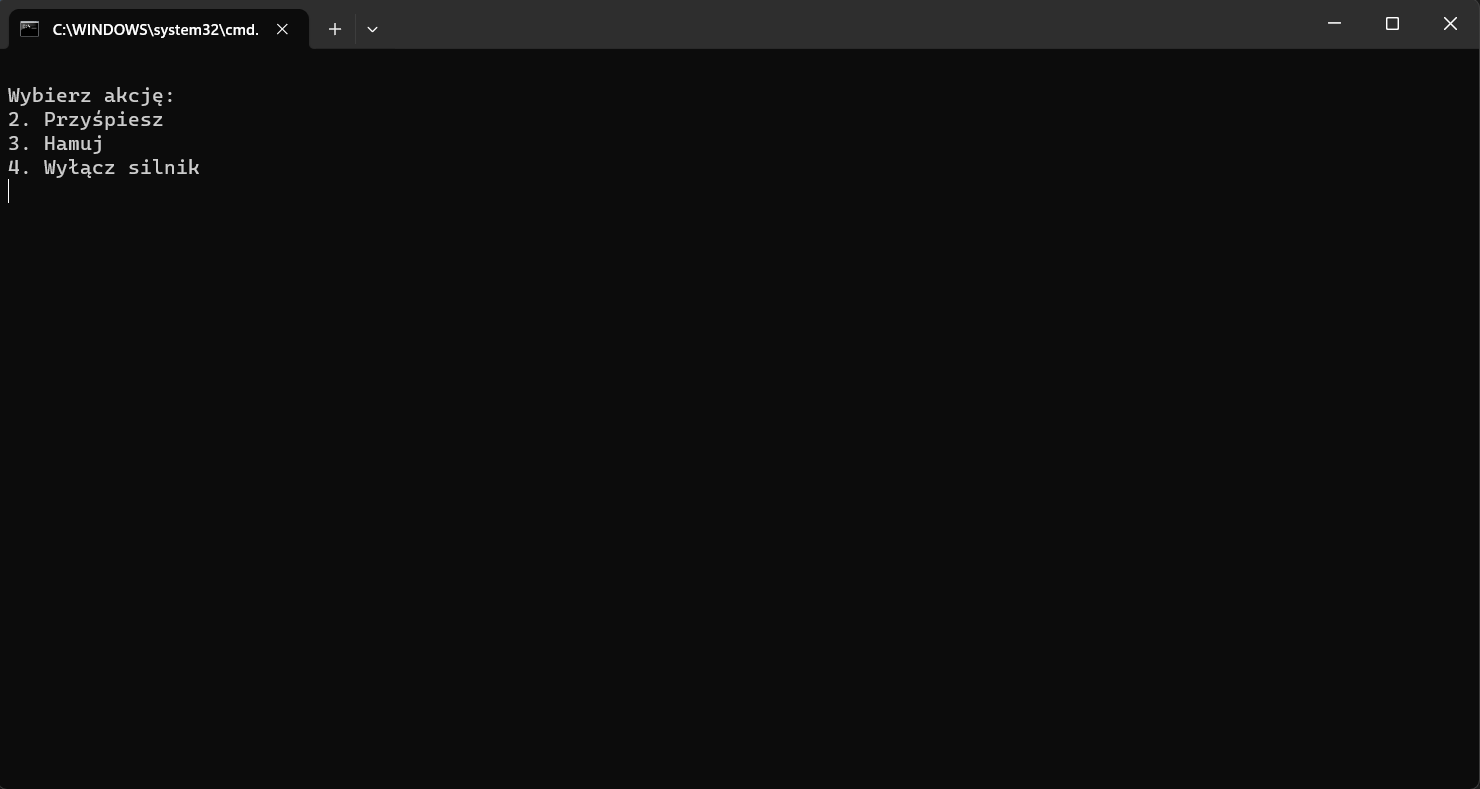
\includegraphics[width=17cm]{Wyłączenie silnika.png}
	\caption{\footnotesize Wyłączenie silnika}
	\label{fig:plotend}
\end{figure}
% ********** Koniec rozdziału **********

\newpage
% ********** Rozdział 4 **********
\chapter{Podsumowanie}
\section{Podsumowanie projektu}

Podsumowując projekt "System Zarządzania Symulacją Samochodu", można stwierdzić, że zostały zrealizowane główne założenia projektu, które obejmowały stworzenie realistycznego doświadczenia jazdy samochodem wraz z możliwością interaktywnego sterowania pojazdem oraz monitorowania kluczowych parametrów. System został zaprojektowany w sposób prosty, czytelny i łatwy dla użytkownika, co pozwoliło na płynną interakcję i maksymalne zrozumienie procesu symulacji. W ramach projektu opracowano również diagram klas, który przedstawił strukturę klas i ich relacje w systemie. Wykorzystano technologie .NET Framework oraz narzędzia takie jak Visual Studio do implementacji projektu. Repozytorium znajduje się na platformie GitHub, co umożliwia monitorowanie kodu. Warstwa użytkowa projektu została zaprezentowana poprzez interaktywną konsolę, która umożliwiała wykonywanie różnych akcji związanych z symulacją samochodu, takich jak włączenie silnika, przyśpieszanie, zmiana biegów, hamowanie, a także monitorowanie parametrów pojazdu, takich jak prędkość, obroty silnika czy stan paliwa. W ramach podsumowania projektu można stwierdzić, że udało się zrealizować postawione cele i założenia, tworząc kompleksowy system do symulacji i analizy zachowania samochodu. 


% ********** Koniec rozdziału **********


% *************** Bibliografia ***************
\begin{thebibliography}{6}
\addcontentsline{toc}{chapter}{Bibliografia}
%dodanie wpisu do spisu bibliograficznego

\bibitem{www-1} https://learn.microsoft.com/pl-pl/visualstudio/releases/2022/system-requirements

\bibitem{etykieta2}https://helion.pl/ksiazki/c-rusz-glowa-wydanie-iv-andrew-stellman-jennifer-greene,cshr4v.htm\#format/d


\end{thebibliography}
\newpage

% *************** Zakończenie ***************
% *************** Zakończenie ***************

%***************************************************************************************
% W tym miejscu znajdują się polecenia odpowiedzialne za tworzenie
% spisu ilustracji, spisu treści oraz streszczenia pracy
%***************************************************************************************

%spis rysunków
\addcontentsline{toc}{chapter}{Spis rysunków}
\listoffigures
\newpage




% *************** Koniec pliku back.tex ***************


\end{document}
% *************** Koniec pliku szablon.tex ***************
